\renewcommand{\theequation}{\theenumi}
\begin{enumerate}[label=\arabic*.,ref=\thesubsubsection.\theenumi]
\numberwithin{equation}{enumi}
%
\item Let $\myvec{1&-1}\vec{x} = 0$ intersects the circle $\norm{\vec{x}} = 1$ at point $\vec{A} = \myvec{a\\b}$ in the first quadrant. The circle $\norm{\vec{x}} = 1$ intersects the x-axis at point $\vec{B} = \myvec{1\\0}$ in the first quadrant.

\begin{align}
\myvec{1&-1}\vec{x} = 0
\\
\myvec{1&-1}\myvec{a\\b} = 0
\\
a=b \label{eq:1}
\\
\norm{\vec{x}} = 1
\\
\sqrt{a^2+b^2} = 1
\\
From \eqref{eq:1},
2a^2 = 1
\\
a = \frac{1}{\sqrt{2}} = b
\end{align}

Finding scalar products,
\begin{align}
\vec{A} = \myvec{\frac{1}{\sqrt{2}}\\\frac{1}{\sqrt{2}}}
\end{align}
\begin{align}
(\vec{A} - \vec{O})^T(\vec{B} - \vec{O}) = \norm{\vec{A} - \vec{O}}\norm{\vec{B} - \vec{O}}\cos{\angle{AOB}}
\\
(\myvec{\frac{1}{\sqrt{2}}\\\frac{1}{\sqrt{2}}})^T(\myvec{1\\0}) = \norm{\myvec{\frac{1}{\sqrt{2}}\\\frac{1}{\sqrt{2}}}} \norm{\myvec{1\\0}} \cos{\angle{AOB}}
\end{align}
\begin{align}
\myvec{\frac{1}{\sqrt{2}}\\0} = 1 \times 1 \times \cos{\angle{AOB}}
\\
\cos{\angle{AOB}} = \frac{1}{\sqrt{2}}
\\
\angle{AOB} = 45\degree
\end{align}

Area of the circle = $\pi \times r^2$
Area of the sector $AOB$:
\begin{align}
\frac{\angle{AOB}}{360}\pi \times r^2
\\
\frac{45}{360}\pi \times 1^2
\\
\frac{\pi}{8}
\\
0.3927 units^2
\end{align}

Required area = Area of the sector $AOB$ = $0.3927$ $units^2$\\ 
The circle in Fig.\ref{fig:cir_1} is generated using the following python code 
\begin{lstlisting}
codes/circle/example/circle.py
\end{lstlisting}

\begin{figure}[!ht]
\centering
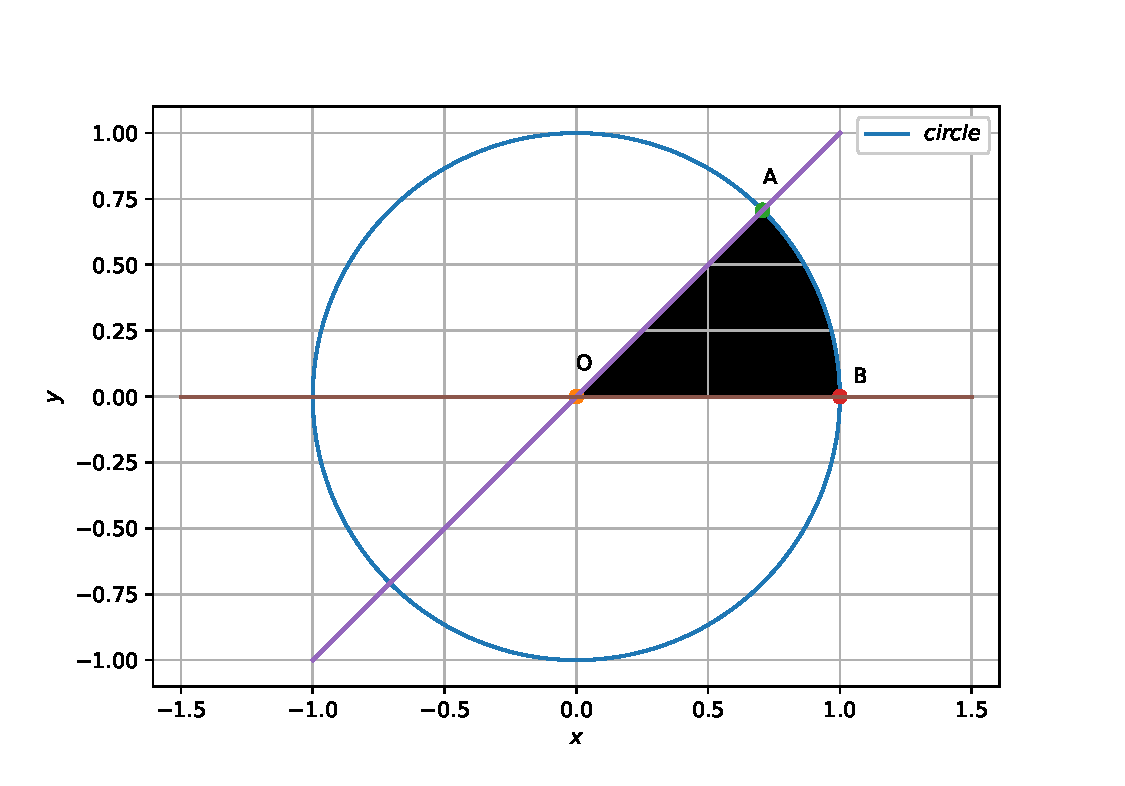
\includegraphics[width=\columnwidth]{./codes/circle/example/circle.eps}
\caption{Circle generated using python}
\label{fig:cir_1}
\end{figure}

\end{enumerate}